% !TEX spellcheck = en_US

% ======================================= V
% (NC) 2019 Haluk Bingol
% github.com/halukbingol/LaTeX-Templates
%
% Licensees may copy, distribute, display, and perform the work and make derivative works 
% and remixes based on it only for non-commercial purposes. 
% ======================================= A




%\documentclass[pre,twocolumn,showkeys,longbibliography,nofootinbib]{revtex4-1}
\documentclass[pre,twocolumn,showkeys,longbibliography]{revtex4-1}
%\documentclass[twocolumn,preprintnumbers,amsmath,amssymb,superscriptaddress,pre]{revtex4}




%: ==== HB Header Common Packages v20160423 ====V
	\usepackage[utf8]{inputenc} % To use Unicode characters
	\usepackage[iso]{datetime}
	%	\usepackage{etex}
	
	\usepackage[a4paper]{geometry}
	
	\usepackage{xcolor}
	% black, blue, brown, cyan, darkgray, gray, green, lightgray, lime, 
	% magenta, olive, orange, pink, purple, red, teal, violet, white, yellow
	\usepackage[colorlinks=true,linkcolor=red,urlcolor=blue,citecolor=red]%
		{hyperref}
	\usepackage{graphicx,epstopdf}
	% \graphicspath{{fig}}
	\graphicspath{{../common/figures/}}
	% \DeclareGraphicsExtensions{.pdf,.jpeg,.png,.eps}
	% \DeclareGraphicsRule{.tif}{png}{.png}%
	%	{`convert #1 `dirname #1`/`basename #1 .tif`.png}
%	\usepackage{subfigure}
%\usepackage{subfig}
\usepackage{subcaption}




%: ==== HB Header Common Declarations v20170816 ====V
	\newcommand{\hbTimeStamp}{{\color{red}--Draft-- v\today/\currenttime}} % version
	%
	\newcommand{\reffig}[1]{Fig.~\ref{#1}}
	\newcommand{\refeq}[1]{Eq.~\ref{#1}}
	\newcommand{\reftbl}[1]{Table~\ref{#1}}
	\newcommand{\refsec}[1]{Sec.~\ref{#1}}
	\newcommand{\refcite}[1]{Ref~\cite{#1}}
	\newcommand{\refalg}[1]{Algorithm~\cite{#1}}
	\newcommand{\reflst}[1]{List.~\ref{#1}}  % code listing
	%
	\newcommand{\refthm}[1]{Theorem~\ref{#1}}
	\newcommand{\refthmA}[2]{\refthm{#1}(\ref{#2}}
	\newcommand{\reflem}[1]{Lemma~\ref{#1}}
	\newcommand{\refdef}[1]{Definition~\ref{#1}}
	\newcommand{\refexmp}[1]{Example~\ref{#1}}
	%
	\newcommand{\hbQuote}[1]{{\small \textsf{``#1''}}}
	%
	\newcommand{\hbCode}[1]{\texttt{#1}}
	%
	\newcommand{\hbIdea}[1]{{\color{olive}{\scriptsize [{#1}]}}}
	\newcommand{\hbFootnote}[2]{\footnote{{\color{red} @#1 : }#2}}
% ==== HB Header Common Declarations ====A




%: ==== HB Header Common Math v20170530 ====V
	% ams
	\usepackage{amsmath, amssymb,amsfonts,amsthm}
	
	\newcommand{\hbVec}[1]{\mathbf{#1}}	% vector
	\newcommand{\hbAbs}[1]{| #1 |}	% absolute value
	\newcommand{\hbNorm}[1]{\left\lVert #1 \right\rVert}	% norm 2
	\newcommand{\hbMat}[1]{\mathbf{#1}}	% matrix
	\newcommand{\hbSet}[1]{\mathcal{#1}}	%
	\newcommand{\argmin}[2]{\underset{#1}{\operatorname{arg \, min}}\;#2}
	\newcommand{\argmax}[2]{\underset{#1}{\operatorname{arg \, max}}\;#2}

	
	\theoremstyle{plain}% default
	\newtheorem{thm}{Theorem}[section]
	\newtheorem{lem}[thm]{Lemma}
	\newtheorem{prop}[thm]{Proposition}
	\newtheorem*{cor}{Corollary}
	\theoremstyle{definition}
	\newtheorem{defn}{Definition}[section]
	\newtheorem{conj}{Conjecture}[section]
	\newtheorem{exmp}{Example}[section]
	\theoremstyle{remark}
	\newtheorem*{rem}{Remark}
	\newtheorem*{note}{Note}
% ==== HB Header Common Math v20170530 ====A




%: == HB Code Listing v20161002 ====V
\usepackage{listingsutf8}
%\usepackage{listings}             % Include the listings-package
\definecolor{hbGreen}{rgb}{0,0.6,0}
\definecolor{hbGray}{rgb}{0.5,0.5,0.5}
\definecolor{hbMauve}{rgb}{0.58,0,0.82}
\definecolor{hbbgColor}{rgb}{0.98,0.98,0.98}
%
\lstset{ %
	backgroundcolor=\color{hbbgColor},   % choose the background color; you must add \usepackage{color} or \usepackage{xcolor}
%  basicstyle=\tiny, % the size of the fonts that are used for the code
	basicstyle=\tiny\ttfamily, % the size of the fonts that are used for the code
%  basicstyle=\scriptsize\ttfamily, % the size of the fonts that are used for the code
%  basicstyle=\footnotesize\ttfamily, % the size of the fonts that are used for the code
	breakatwhitespace=false,         % sets if automatic breaks should only happen at whitespace
	breaklines=true,                 % sets automatic line breaking
	captionpos=b,                    % sets the caption-position to bottom
	commentstyle=\color{hbGreen},    % comment style
	deletekeywords={...},            % if you want to delete keywords from the given language
	escapeinside={\%*}{*)},          % if you want to add LaTeX within your code
	extendedchars=true,              % lets you use non-ASCII characters; for 8-bits encodings only, does not work with UTF-8
	frame=single,                    % adds a frame around the code
	keepspaces=true,                 % keeps spaces in text, useful for keeping indentation of code (possibly needs columns=flexible)
	keywordstyle=\color{blue},       % keyword style
	language=Sh,                     % the language of the code
	morekeywords={*,...},            % if you want to add more keywords to the set
	numbers=left,                    % where to put the line-numbers; possible values are (none, left, right)
	numbersep=5pt,                   % how far the line-numbers are from the code
	numberstyle=\tiny\color{hbGray}, % the style that is used for the line-numbers
	rulecolor=\color{black},         % if not set, the frame-color may be changed on line-breaks within not-black text (e.g. comments (green here))
	showspaces=false,                % show spaces everywhere adding particular underscores; it overrides 'showstringspaces'
	showstringspaces=false,          % underline spaces within strings only
	showtabs=false,                  % show tabs within strings adding particular underscores
	stepnumber=2,                    % the step between two line-numbers. If it's 1, each line will be numbered
	stringstyle=\color{hbMauve},     % string literal style
	tabsize=1,                       % sets default tabsize to 2 spaces
	title=\lstname                   % show the filename of files included with \lstinputlisting; also try caption instead of title
	literate={├}{|}1 {─}{--}1 {└}{+}1
}
\lstset{basicstyle=\ttfamily}
% == HB Code Listing v20161002 ====A




%: ==== HB Track Changes v20170522 ====V
	\usepackage{changes}
	% black, blue, brown, cyan, darkgray, gray, green, lightgray, lime, 
	% magenta, olive, orange, pink, purple, red, teal, violet, white, yellow
	
	\definechangesauthor[name=Haluk Bingol,color=purple]{hb}
	\definechangesauthor[name=Aaaa Bbbb,color=blue]{ab}
	\setremarkmarkup{(#2)}
	
	%\listofchanges    % track changes use at the bottom
	
	% ==== usage
	
	%\added[id=hb]{
	%	aaa
	%}
	
	%\replaced[id=hb]{
	%	aaa
	%}{
	%	bob
	%}
	
	%\deleted[id=hb]{
	%	aaa
	%}

	%\added[id=hb]{newText}
	%\added[id=hb,remark={yourRemark}]{newText}
	%\deleted[id=hb]{deletedText}
	%\deleted[id=hb,remark=yourRemark]{deletedText}
	%\replaced[id=hb]{newText}{deletedText}
%  ==== HB Track Changes v20170522 ====V



%: ======= specific ===============
% frequently used terms
\newcommand{\hbDTex}{\hbCode{.tex}}
\newcommand{\hbDPdf}{\hbCode{.pdf}}
\newcommand{\hbSSpecific}{\hbCode{specific}}


\DeclareGraphicsExtensions{.png}
%
\DeclareMathOperator{\sgn}{sgn}
\DeclareMathOperator{\cov}{cov}
%
%\newcommand{\hbAvg}[1]{\widehat{#1}}
\newcommand{\hbOpt}[1]{{#1}^*}

\newcommand{\hSoX}{\mathbb{X}} % generic set
\newcommand{\hSoN}{\mathbb{N}} % the set of natural numbers
\newcommand{\hSoR}{\mathbb{R}} % the set of real numbers

% ======= specific ===============









%\usepackage{lineno,hyperref}
%\modulolinenumbers[5]

%\usepackage{lineno}
%\usepackage[switch,columnwise]{lineno}
\RequirePackage{lineno}
%\linenumbers 


% ========================================
\begin{document}

%\setpagewiselinenumbers
%\modulolinenumbers[5]
%\linenumbers



\title{
	My \LaTeX\ Paper Template 
}
\author{Haluk O. Bingol}

\affiliation{
	Department of Computer Engineering,\\
	Bogazici University\\
	Istanbul, Turkey\\
	bingol@boun.edu.tr
}
%\date{\today}
\date{\hbTimeStamp}

\begin{abstract}
	This is my \LaTeX\ template for paper.
\end{abstract}


% ========================================
\keywords{
	LateX paper template;
	keywordB;
	keywordC;
}


% ========================================
\maketitle
\tableofcontents

%\linenumbers




% ========================================
\section{Introduction}

This is my paper template. 
It is developed by experience, necessities, best practices.





% =======================================
\section{\LaTeX\ source code conventions}

Consider \LaTeX\ code as programming language code. 
Actually it is a programming language.





% =======================================
\subsection{left start}

Start your line at the left most position.
Do not indent paragraphs unless they are nested within a structure such as \verb!begin-end! block.
So indentation should be used properly.




% =======================================
\subsection{Keep the line length short}

Some editors organize one paragraph of \LaTeX\ code as one line.
Try not to use such an editors.
The lines should be short.
There are two advantages for shorter lines.
\begin{enumerate}

	\item
	\LaTeX\ works on line.
	Any error message it produces provide you a line number. 
	If the line is a long one,
	it is harder to locate the error.

	\item
	Many version control system such as git works on line as prime object.
	Any change in a line is tracked.
	If the line is too long,
	tracking gets more space since entire line has to be considered.

\end{enumerate}
If line gets too long,
divide it by a ``return'' at a proper point.
A possible places to break the line are ``that'', ``where'', ``which'' phrases or ``else'' part of ``if''. 




% =======================================
\subsection{Usage of space and indentation}

Use space and indentation freely so that your source code would be easy to read and maintain.
For example use 4 empty line and followed by a comment before section separators.
See the source code of this paragraph.
See also the source code of the previous ``enumerate'' block.

In math mode, 
use spaces to increase readablility.
For example, see the source code of this in line math equation.
This is binomial number
$
	a = {n \choose r}
$
with smart usage of spaces.
The similar smart space usage can be seen in this math display format, too.
\begin{align}
	\bar{a} 
		= 
			\frac{1}{\hbAbs{A}}
			\sum_{i \in A} a_{i}
		= 5.
\end{align}

Using math and not math mode.
If you are talking about a variable,
use math mode such as $a$.
Any numeric value is recommended to be in math mode.
Notice that -1 in text mode is quite different than $-1$ in math mode.
Use $k$-means, rather than $k-$means.




% =======================================
\section{Header Part}

Note that timestamp \hbTimeStamp\ that helps to keep track of versions while the paper is developed.
Do not forget to remove it before submission.




% =======================================
\subsection{TexShop Specific}

I use TexShop.
It has some features that I use.
\begin{itemize}

	\item
	Tag list feature of TeXShop enables you to directly go to a segment of your document.
	Sections are automatically listed in here.
	I need to extend that for my purposes.
	A \LaTeX\  comment starts with ``\hbCode{\%}''.
	If comment starts with`` \hbCode{\%:}'',
	note the additional ``\hbCode{:}'',
	then it is listed in the tags list, too.
	I use this feature to fast access to some parts of the document such as figures and tables.
	So I add comments such as 
	``\hbCode{\%: -fig.1}'' for figure 1 and
	``\hbCode{\%: -tbl 3}'' for table 3.
	
	\item 
	\hbCode{\% !TEX spellcheck = en\_US} forces the spellchecker to use American English.
	
\end{itemize}





% =======================================
\subsection{Common Packages}




% =======================================
\subsection{Common Declarations}




% =======================================
\subsection{Specific}

Anything that is specific to this paper should be defined in \hbSSpecific\ in the header.




% =======================================
\section{Multi-Author Case}

Usually more than one author involved.
They have to keep track of changes, leave messages to each other
while the paper developes.

Suppose we have two authors, namely HB and AB.
Note that you need to modify 
\hbCode{definechangesauthor}
in 
\hbCode{changes} package.
You may want to set different colors, too.



% =======================================
\subsection{Track Changes}

Authors should be able to add, delete and change parts of the document.
\deleted[id=hb]{
	HB removes this part.
}
\added[id=ab]{
	AB adds this part.
}
HB wants to replace some part with some others as
\replaced[id=hb]{
	the new text
}{
	the old text
}




% =======================================
\subsection{Communicate with Footnotes}

Another way to communicate between authors is to use of footnotes
\hbFootnote{HB}{
	This is a footnote by HB.
}.
The other author has another footnote
\hbFootnote{AB}{
	This is a footnote by AB.
}
.
Note that this is not the same as regular footnotes that you intent to keep in your final document such as~\footnote{
	This is a footnote that should stay in the final version of the document.
}.
These communication footnotes should be removed at the end of development process.
Color of ``@HB'' at the start of the footnote should warn you, if you are looking the \hbDPdf\ file online.
One final search in the \hbDTex\ file for ``@'' should help you to locate unremoved ones.






% =======================================
\subsection{Lists}

This is an enumeration.
\begin{enumerate}

	\item 
	\textbf{Aaaa.}
	Describe Aaaa.

	\item 
	\textbf{Aaaa.}
	Describe Aaaa.

\end{enumerate}




% ========================================
\section{Math}

Please note the usage of spaces while writing math in \hbDTex\ file.
Proper usage of space will improve readability of your \LaTeX\ code.

This is math in line. 
The row sum of $i$ is given as
$
	a_{k \cdot} = \sum_{j=1}^{N} a_{i j}
$,
where $A = [a_{i j}]$ is a matrix.

If you want your math in display mode there are two options. 
If you are not going to refer it again, 
use \verb!\[ ... \]!, 
which produces
\[
	e_{\mu x} 
	= \frac{a_{\mu x}}{\sum_{x'=1}^{S} a_{\mu x'}},
	\quad
	d_{x \mu} 
	= \frac{a_{\mu x}}{\sum_{\mu'=1}^{M} a_{\mu'x}}.
\]
If you are going to refer it again, 
use \verb!\begin{align} ... \end{align}! to obtain
\begin{align}
	a_{ij} =
		\frac{1}{M}
		\sum_{\mu = 1}^{M} 
		{\sum_{x = 1}^{S} 
			e_{\mu x}^{(i)}
			d_{x \mu}^{(j)} }.
	\label{eq:aij}
\end{align}
If you have multiple line derivation,
then \hbCode{align} with \verb!&! is the solution.
\begin{align}
	a 
	&= bbbbb\\
	&= cccc\\
	&= ddd.
\end{align}
If you do not refer the equation later,
get rid off numbers by using 
\verb!\begin{align*} ... \end{align*}!
as
\begin{align*}
	a 
	&= bbbbb\\
	&= cccc\\
	&= ddd.
\end{align*}







% =======================================
\subsection{Referring to an Equation}

Refer an equation \refeq{eq:aij}.
You can refer to an equation \refeq{eq:kBar} in the appendix, too.




% =======================================
\subsection{Subscripts and superscripts}

Always use curly brackets when you use subscripts or superscripts 
even if there is no need due to single symbol.
For example \verb!a_{i}! is better than \verb!a_i! 
if you consider
\verb!a_{ij}! and \verb!a_ij!.
They produce
$a_{i}$,
$a_i$,
$a_{ij}$, and 
$a_ij$,
respectively.




% ========================================
\subsubsection{Comprehension}

Suppose agent $i$ wants to pass meaning $\mu$ to agent $j$.
Probability of doing this correctly is
\[
	\sum_{x = 1}^{S} 
		e_{\mu x}^{(i)}
		d_{x \mu}^{(j)} 
\]
where 
$e_{\mu x}^{(i)}$
and 
$d_{x \mu}^{(j)}$
are encoding of $i$ 
and decoding of $j$, 
respectively.
When we average that over all meanings,
we obtain \emph{comprehension} from $i$ to $j$, 
that is
If we want them to communicate both ways,
we consider \emph{mutual comprehension}
\[
	aaa{\hbSet{C}} = 	
	\frac{1}{2 {\hbAbs{\hbSet{C}} \choose 2}} 
	\sum_{i \in \hbSet{C}}
	\sum_{
		\substack{
			j \in \hbSet{C}\\
			j \neq i
		}
	} 
	{bb{i}{j}}.
\]





% ========================================
\subsection{$k$-means Clustering Algorithm}





% =======================================
\subsubsection{Finding Optimum Language Clusters}


\[
	Aaaa{K} =
		\argmax
			{K}
			{bbb{\mathbb{P}_{K}}}.
\]






% ========================================
\section{Figures}

Refer to a figure as \reffig{fig:FigWP.eps}.
If you want to refer to a figure with multiple graphs,
there is a way to refer all at once \reffig{fig:N100},
 or individually \reffig{fig:FigWStar} and \reffig{fig:FigKStar100} as required.






% +++++++++++++++++++++++++++++++++++++++
%: -fig.1
\begin{figure}[!tbp]
	\centering 
	\includegraphics[width=\columnwidth]%
		{Fig-IStar.eps}
	\caption{
		Single figure.
	} 
	% \caption
	\label{fig:FigWP.eps}
\end{figure}
% +++++++++++++++++++++++++++++++++++++++


% +++++++++++++++++++++++++++++++++++++++
%: -fig 2
\begin{figure}[!tbp]
	\begin{subfigure}{\columnwidth}%
		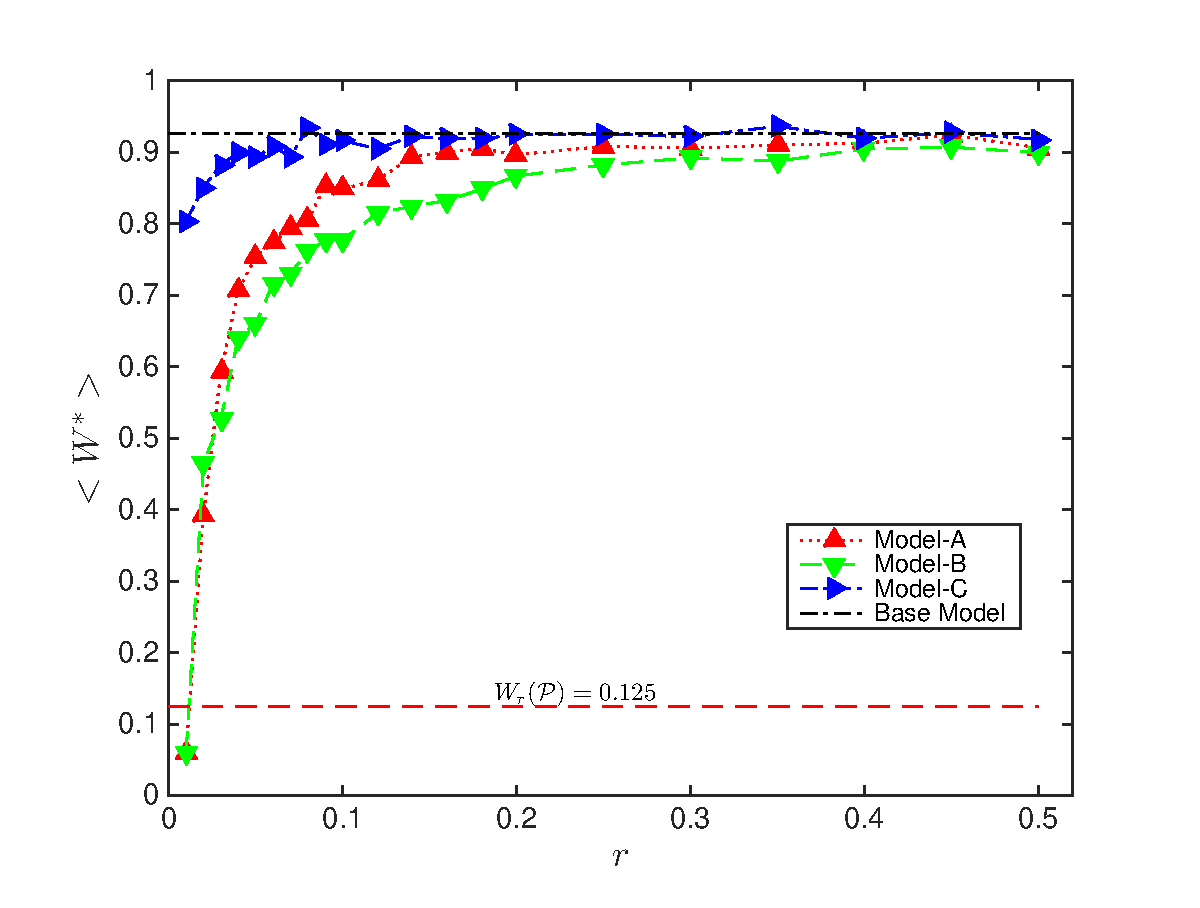
\includegraphics[width=\columnwidth]
			{Fig-WStar.eps}
		\caption{Within Community Comprehensions} 
		\label{fig:FigWStar}
	\end{subfigure}
	\begin{subfigure}{\columnwidth}%
		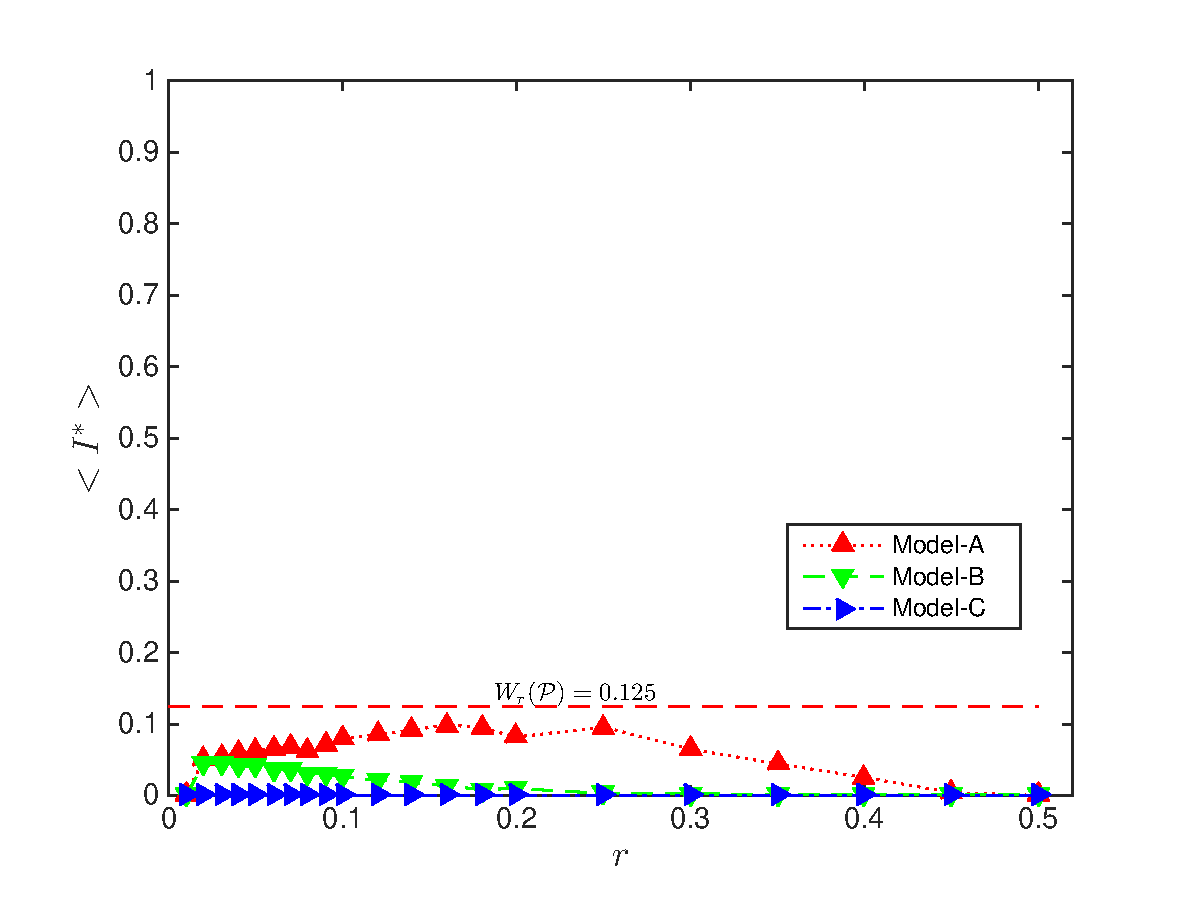
\includegraphics[width=\columnwidth]
			{Fig-IStar.eps}
		\caption{Inter-Community Comprehensions} 
		\label{fig:FigIStar}
	\end{subfigure}
	\begin{subfigure}{\columnwidth}%
		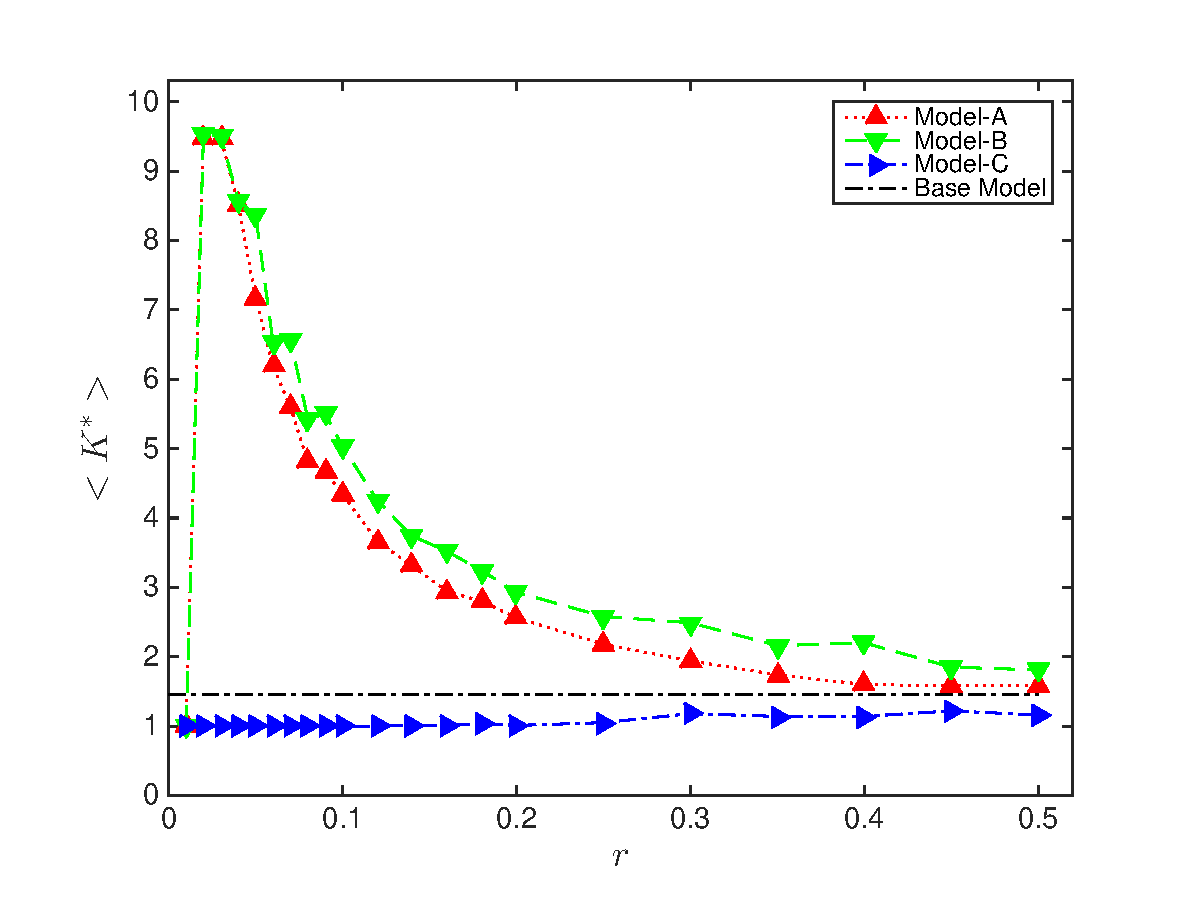
\includegraphics[width=\columnwidth]
			{Fig-KStar100.eps}
		\caption{Subcommunity Counts} 
		\label{fig:FigKStar100}
	\end{subfigure}
	\caption{
		Language subcommunities.
		$N = 100$.
	} % \caption
	\label{fig:N100}
\end{figure}
% +++++++++++++++++++++++++++++++++++++++






% ========================================
\section{References and citations}
\label{sec:ReferencesAndCitations}

Journals may have different ways to present references. 
If one use consistently the same macro for references,
simple change in the macro definition can solve 
the problem of adjusting from one journal to another.
There are a number of objects such as 
definitions \refdef{def:PositiveIntegerPowers}, 
examples \refexmp{exp:Generic},
figures, 
code listings \reflst{lst:QuickStart}
 that you can refer to.

% ========================================
\begin{defn}[Positive Integer Powers]
	For all $x \in \hSoX$, and $n \in \hSoN$
	\[
		x^{n} \triangleq
		\begin{cases}
			1, 
			 &n = 0, \\
			x, 
			 &n = 1, \\
			x x^{n-1},
			 &n > 1.
		\end{cases}
	\]
	\label{def:PositiveIntegerPowers}
\end{defn}

% ========================================
\begin{exmp}
	\label{exp:Generic}
	Note that $\hSoX$ is defined in a very generic way.
	We can take $\hSoX$ as 
	natural numbers $\hSoN$,
	real numbers $\hSoR$, or
	$N \times N$ real matrices $\hSoR_{N \times N}$.
\end{exmp}

% ========================================
\lstinputlisting[language=java,basicstyle=\tiny\ttfamily,label=lst:QuickStart,caption=Node object]
	{code-sample.java}




% ========================================
\subsection{References}

Any object that will be referred,
should have a label declaration such as
\verb!\label{A:B}!,
where 
$A$ is type indicator and
$B$ is unique label with in the type.
Commonly used type indicator are given in \reftbl{tbl:TypeIndicators}.
See ``HB Header Common Declarations'' in the source for more.



% +++++++++++++++++++++++++++++++++++++++
%: -table TypeIndicators
\begin{table}[th]
	\caption{Reference type indicators}
	\begin{center}
	\begin{tabular}{|l |l |l |l |}
		\hline
		Type
		&Indicator
		&Code
		&Result\\
		\hline
		%
		Equation
		&eq
		&\verb!\refeq!
		&\refeq{eq:kBar}\\
		%
		Figure
		&fig
		&\verb!\reffig!
		&\reffig{fig:FigIStar}\\
		%
		Table
		&tbl
		&\verb!\reftbl!
		&\reftbl{tbl:gamma}\\
		%
		Section
		&sec
		&\verb!\refsec!
		&\refsec{sec:kMeansAlgorithm}\\
		%
		Citation
		&-
		&\verb!\refcite!
		&\refcite{duda2012pattern}\\
		%
		Definition
		&def
		&\verb!\refdef!
		&\refdef{def:PositiveIntegerPowers}\\
		%
		Theorem
		&thm
		&\verb!\refthm!
		&\refthm{aa}\\
		%
		Algorithm
		&alg
		&\verb!\refalg!
		&\refalg{aaa}\\
		%
		List
		&lst
		&\verb!\reflst!
		&\reflst{lst:QuickStart}\\
		%
		aaa
		&aaa
		&\verb!aaaa!
		&aaa\\
		\hline
	\end{tabular}
	\end{center}
	\label{tbl:TypeIndicators}
\end{table}%
% +++++++++++++++++++++++++++++++++++++++


It is possible to refer a number of objects within \LaTeX.
Refer an equation \refeq{eq:aij}, which can be obtained by \verb!\refeq{eq:aij}!. 
A figure can be referred by means of \verb!\reffig{fig:N100}!, which produces \reffig{fig:N100}.
Similarly a table can be referred by \reftbl{tbl:gamma} by using \verb!\reftbl{tbl:gamma}!.
A section can be referred by \refsec{sec:ReferencesAndCitations}, 
that is, 
\verb!\refsec{sec:ReferencesAndCitations}!.



% ========================================
\subsection{Citations}

Check the source to see how I prefer to cite~\cite{%
	duda2012pattern,
	mackay2003information,
	theodoridis2010patternMatlab}.
In this way, you can see the citations easily both in .tex and .pdf forms.
In .pdf file, citations are in color.
If you want to modify,
see 
\hbCode{linkcolor=red}
in 
\hbCode{hyperref}.
Use citation at  the end of sentence as much as possible.
Connect citation to the word with tilda as in the case here~\cite{%
	AAa2017bb}.
See the code.
If a sentence starts with citation,
start with~\refcite{%
	AAa2017bb}  
not with~\cite{%
	AAa2017bb}.









% =======================================
\subsection{Tables}


Refer to tables as \reftbl{tbl:gamma}.


% +++++++++++++++++++++++++++++++++++++++
%: -table 1
\begin{table}[th]
	\caption{$\gamma$ values for $r > 0.03$}
	\begin{center}
	\begin{tabular}{|r|cc|}
		\hline
		$N$
		&Model-A %\quad
		&Model-B\\
		\hline
		%
		50
		&0.72
		&0.62\\
		%
		100
		&0.69
		&0.63\\
		%
		150
		&0.72
		&0.69\\
		%
		200
		&0.68
		&0.72\\
		\hline
	\end{tabular}
	\end{center}
	\label{tbl:gamma}
\end{table}%
% +++++++++++++++++++++++++++++++++++++++





% =======================================
\appendix
%: ==== HB Header Common for Appendix v20170517 ====V
\newcommand{\hbAppendixPrefix}{A}
%
\renewcommand{\thefigure}{\hbAppendixPrefix\arabic{figure}}
\setcounter{figure}{0}
\renewcommand{\thetable}{\hbAppendixPrefix\arabic{table}} 
\setcounter{table}{0}
\renewcommand{\theequation}{\hbAppendixPrefix\arabic{equation}} 
\setcounter{equation}{0}
% ==== HB Header Common for Appendix v20170517 ====A

\section{Appendix}
\label{sec:appendix}




% =======================================
\subsection{$k$-means Algorithm}
	\label{sec:kMeansAlgorithm}

An equation
\begin{equation}
	\label{eq:kBar}
	\bar{k} = \argmin{k} d(\mathbf{x}_{n},  \mathbf{m}_{k}(t-1))
\end{equation}
is here.





% =======================================
\subsection{$k$-means in Language Domain}







%% =======================================
\section*{Acknowledgments}

%\textbf{Acknowledgments.}
This work was partially supported 
by Bogazici University Research Fund [BAP-2008-08A105], 
by the Turkish State Planning Organization (DPT) TAM Project [2007K120610], 
and 
by COST action TD1210.




% ========================================
\bibliographystyle{ieeetr}

\bibliography{bingol-template-paper}



% =========
\listofchanges   % track changes use at the bottom
% =========



\end{document}






